\newpage
\section{Generatory liczb losowych}
Na początku każdego przebiegu symulacji tworzona jest instancja generatora liczb losowych \emph{StdRng}.
Ziarno każdego generatora jest losowane ze źródeł zapewnionych przez dany system operacyjny na podstawie jego entropii. Histogramy generowanych liczb losowych z rozkładu równomiernego i wykładniczego przedstawiono na rysunku \ref{rng_hist}.
Ponieważ każda iteracja symulacji musi posiadać niezależny stan wewnętrzny, aby umożliwić wykonywanie równoległe przebiegów, każda iteracja posiada osobny generator liczb losowych z indywidualnie wygenerowanym ziarnem. To rozwiązanie umożliwia także wyznaczanie parametrów statystycznych na podstawie uzyskanych wyników z wielu, krótkich przebiegów, metodą niezależnych replikacji (ang. \emph{independent replication method}). Wymaga ona aby faza początkowa, w której system przechodzi do stanu ustalonego, była krótka względem całkowitego czasu eksperymentu. Tą własność potwierdzono eksperymentem opisanym w sekcji \ref{initial_phase_section}.

\begin{figure}[h]
\center
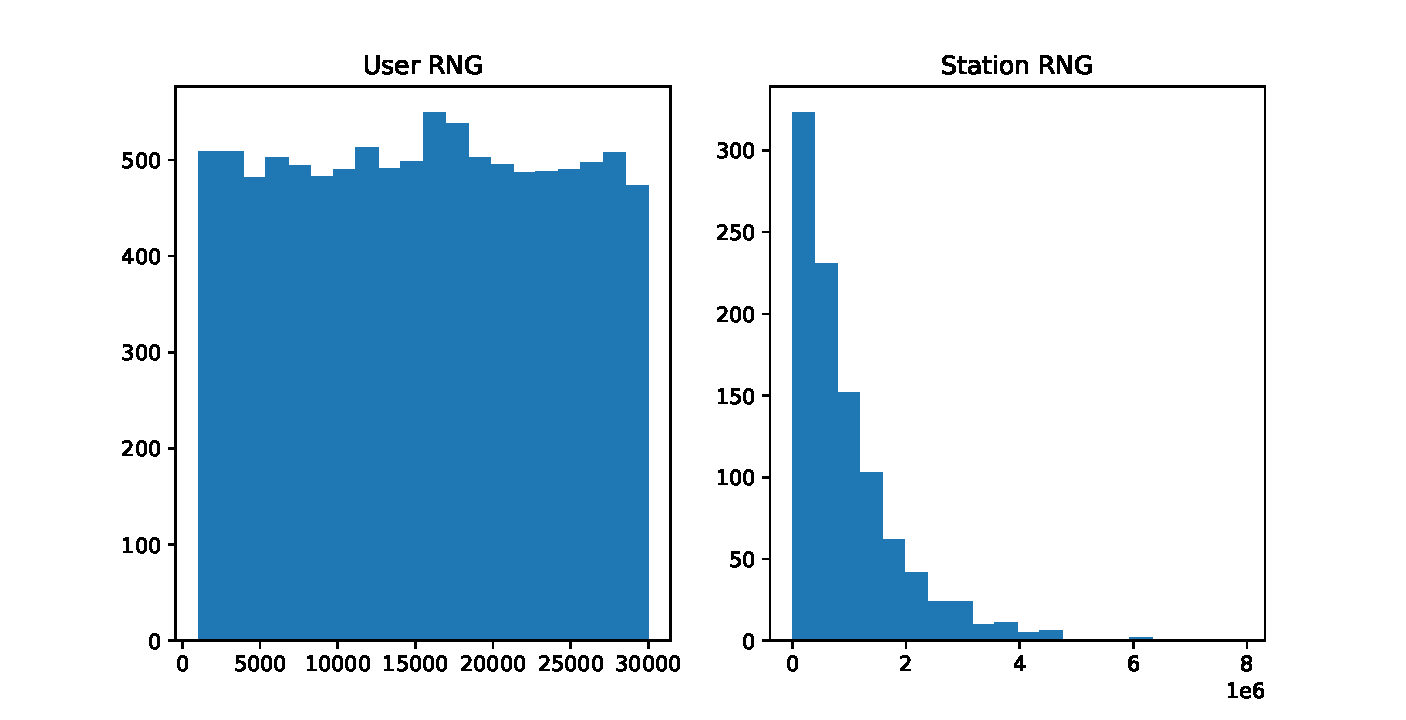
\includegraphics[scale=0.65]{img/rng.pdf} 
\caption{Histogramy reprezentujące generatory liczb losowych czasu przetwarzania użytkownika (\emph{User RNG}) oraz czasu do pojawiania się nowego użytkownika (\emph{Station RNG})}
\label{rng_hist}
\end{figure}